\subsection{Framework Web - Grails}

Nesta secção pretende-se descrever as características da \textit{framework web Grails}, e explicitar as razões que levaram à escolha da mesma para o desenvolvimento da plataforma \textit{BillMate}.

O \textit{Grails} é uma \textit{framework web}, de código aberto, que incorpora o padrão de desenvolvimento \textit{MVC} e que defende o paradigma de convenção em detrimento da configuração, para a linguagem \textit{Groovy}. O seu principal objetivo é ser uma \textit{framework} de alta produtividade, e para isso utiliza as \textit{frameworks} \textit{Hibernate} e \textit{Spring}.

O \textit{Grails} é construido sobre a linguagem \textit{Java}. Essa característica permite que a sua integração com bibliotecas e \textit{frameworks} \textit{Java} seja natural.

Uma das principais vantagens na sua utilização é o grande conjunto de \textit{plugins} que esta disponibiliza e que permitem acelerar significativamente o processo de desenvolvimento.\\

\textbf{\large{Groovy}}\\

O \textit{Groovy} é uma linguagem de programação orientada aos objetos desenvolvida como alternativa à linguagem de programação \textit{Java} e que apresenta características do \textit{Python}, \textit{Ruby} e \textit{Smalltalk}. É uma linguagem que pretende oferecer mecanismos que não estão presentes no \textit{Java} e melhorar a legibilidade do código produzido.\\

\textbf{\textit{Arquitetura}}\\

\begin{figure}[H]
\centerline{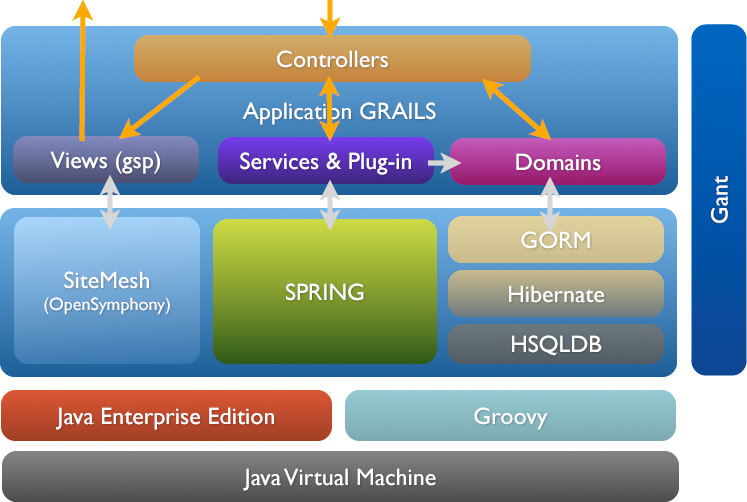
\includegraphics[width=.5\textwidth]{images/implementation/architecture_grails}}
\caption{Arquitetura Grails}
\label{fig:arqgrails}
\end{figure}

\hspace{1cm}

A figura \ref{fig:arqgrails} apresenta a arquitetura de uma aplicação \textit{Grails}. A sua estrutura será indicada na seguinte lista com mais detalhe.

\begin{itemize}
    \item \textbf{\textit{Domain classes}}\\

    As \textit{domain classes} são dos componentes mais importantes de uma aplicação \textit{web} em \textit{Grails}. Cada \textit{domain class} vai corresponder a uma entidade do sistema, estas entidades são normalmente persistidas e estão associadas a uma tabela da base de dados.

    No contexto de uma aplicação \textit{Java Enterprise Edition (JEE)} e utilizando componentes \textit{Enterprise Java Beans (EJB)}, as \textit{domain classes} poderiam representar \textit{entity beans}.

    \item \textbf{\textit{Controllers}}\\

    Os controladores, à semelhança de outras \textit{frameworks web MVC}, são responsáveis por enviar e receber dados das \textit{views} e gerir redirecionamentos e respostas. Estas classes comunicam com as \textit{domain classes}, com os \textit{services} e com as \textit{views}.

    \item \textbf{\textit{Views}}\\

    As \textit{views} são os componentes responsáveis por apresentar dados ao utilizador.

    Para facilitar a integração de conteúdo dinâmico com conteúdo estático, o \textit{Grails} utiliza \textit{Groovy Server Pages (GSP)} que é uma linguagem de apresentação semelhante ao \textit{Java Server Pages (JSP)}.

    \item \textbf{\textit{Services}}\\

    O \textit{Grails} utiliza os \textit{services} para separar a lógica de negócio dos restantes componentes.

    Os \textit{services} podem facilmente fazer uso de funcionalidades de injeção de dependências e são facilmente acessíveis a partir dos controladores.

    No contexto de uma aplicação \textit{Java Enterprise Edition (JEE)} e utilizando componentes \textit{Enterprise Java Beans (EJB)}, as \textit{domain classes} poderiam representar \textit{session beans}.

    \item \textbf{\textit{Tag libraries}}\\

    As \textit{tag libraries} são classes que funcionam como \textit{helpers} para a geração de conteúdo dinâmico nas \textit{views}.

\end{itemize}

\textbf{\large{Spring}}\\

  Como referido anteriormente o \textit{Grails} tem a \textit{framework} \textit{Spring} embebida.

  Este acaba por se definir como uma aplicação \textit{Spring MVC} "disfarçada", tal como é indicado na sua documentação oficial.

  Consequentemente a \textit{framework} utiliza os mecanismos de gestão de \textit{beans} do \textit{Spring}.

  \textbf{\textit{Spring beans}}\\

  Por omissão os \textit{spring beans} são \textit{singletons}, ou melhor, apenas uma instância de cada \textit{bean} é criada.

  No entanto esta omissão nem sempre é a mais indicada, principalmente quando queremos \textit{beans} mutáveis, pelo que é possível definir um \textit{scope} para o referido \textit{bean}.

  O Spring suporta cinco \textit{scopes}:

  \begin{itemize}
    \item \textbf{singleton}

      Como referido, apenas uma instancia é criada criada e disponibilizada no \textit{Spring IoC container}. Sempre que o \textit{bean} é invocado, é sempre a mesma instância que é disponíbilizada.

    \item \textbf{prototype}

      Permite receber uma nova instância do \textit{bean} de cada vez que ele é invocado. Com este \textit{scope} já é possível ter estados mutáveis nos beans, uma vez que cada invoção recebe uma cópia diferente do objeto.

    \item \textbf{request}

      Atribui uma instância por ciclo de vida de um \textit{HTTP request}, o que significa que para cada pedido uma nova instância do \textit{bean} será criada.

    \item \textbf{session}

      Uma nova instância é criada por ciclo de vida de uma \textit{HTTP session}.

    \item \textbf{global}

      Abribui uma instância por ciclo de vida de uma \textit{global HTTP session}.

  \end{itemize}

\pagebreak

\textbf{\large{Hibernate e GORM}}\\

  Como referido anteriormente o \textit{Grails} tem a \textit{framework Hibernate} integrada.

  Para fazer o mapeamento entre o paradigma relacional e o dos objetos o \textit{Grails} oferece um mecanismo baseado em \textit{Hibernate}, que é o \textit{Grails Object Relational Mapping (GORM)}.

  O \textit{GORM} oferece várias facilidades em relação ao \textit{Hibernate}. No \textit{GORM} não é necessário utilizar anotações ou extender classes especiciais para tornar a classe persistente. No \textit{GORM} cada \textit{domain class} representa uma tabela na base de dados e cada atributo representa uma coluna das referidas tabelas.

  O \textit{GORM} oferece assim um nível de abstração superior. Este não é mais do que uma interface (\textit{Facade}) para o \textit{Hibernate}.
